%%%%%%%%%%%%%%%%%%%%%%%%%%%%%%%%%%%%%%%%%
% Kieker Analysis Component
%
% $Date$
% $Rev$:
% $Author$

\chapter{\KiekerAnalysisPart{} Component}\label{chap:componentsAnalysis}

\NOTIFYBOX{The Java sources of this chapter, as well as a pre-compiled binary, %
can be found in the %
\file{\customComponentsBookstoreApplicationDirDistro{}/} directory of the %
binary release.}

\section{Pipe-and-Filter Framework and Included Plugins}\label{sec:analysis:controller}

\KiekerAnalysisPart{} provides a framework to define and execute pipe-and-filter %
architectures of analysis plugins, i.e., monitoring readers and analysis filters, %
as well as repositories. %
This section describes how to use and develop readers, filters, and %
repositories. The description is based on the example %
pipe-and-filter architecture shown in Figure~\ref{fig:example:pipe-and-filter}. The custom monitoring reader %
\class{MyPipeReader}, which corresponds to the writer developed in Section~\ref{sec:monitoring-log-writers}, %
sends records to the connected custom filter \class{MyResponseTimeFilter}. %
This filter accepts only events of the record type \class{MyResponseTimeRecord},
developed in Section~\ref{sec:componentsMonitoring:monitoringRecords}. %
The \class{MyResponseTimeFilter} classifies incoming \class{MyResponseTimeRecord}s %
based on whether they satisfy or exceed a configured threshold and passes them %
to the respective output ports, \method{validResponseTimes} or \method{invalidResponseTimes}. %
Two instances of a second custom filter, \class{MyResponseTimeOutputPrinter}, %
print the received records to the standard output stream.

\begin{figure}
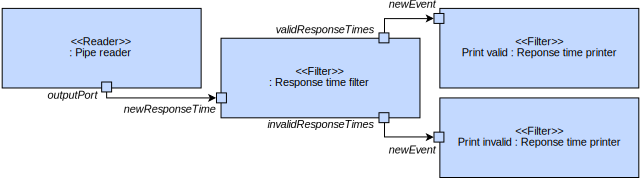
\includegraphics[width=\textwidth]{images/example-pipe-and-filter}
\caption{Example pipe-and-filter configuration}
\label{fig:example:pipe-and-filter}
\end{figure}

%  requires a monitoring reader %
% (Section~\ref{sec:analysis:reader}) and at least %
% one monitoring record consumer plugin (Section~\ref{sec:analysis:consumer}). %
% In addition to the monitoring record consumer plugin, %
% other analysis plugins can be registered. %

\begin{figure}\centering
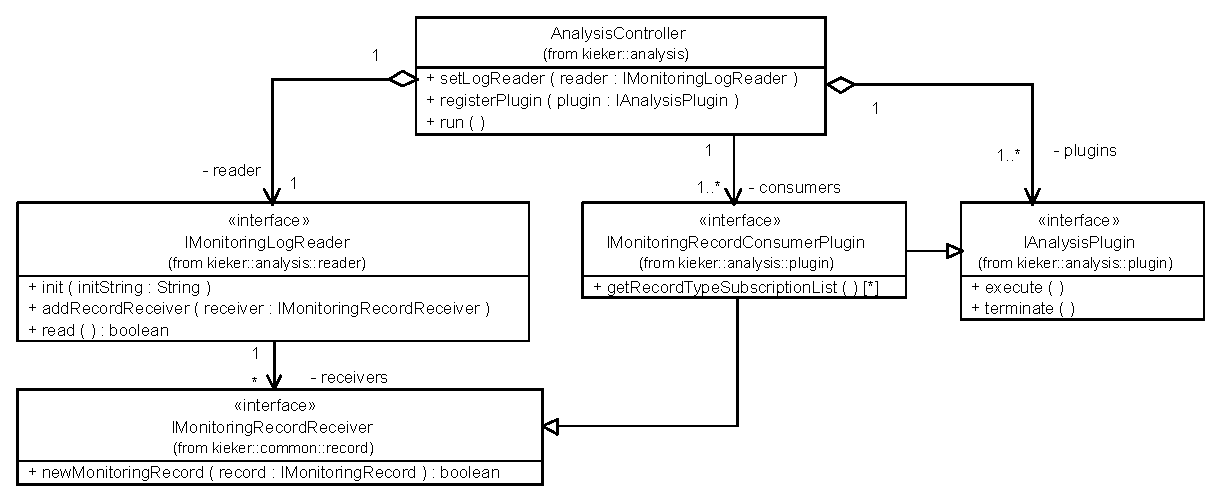
\includegraphics[width=0.95\textwidth]{images/kieker_AnalysisControlleruserguide-modified}
\caption{Class diagram showing important \KiekerAnalysisPart{} classes and their relationship}
\label{fig:analysisController:classdiagram}
\end{figure}

\pagebreak

\noindent Figure~\ref{fig:analysisController:classdiagram} shows the class diagram %
with the important \KiekerAnalysisPart{} classes and their relationships. %
An analysis with \KiekerAnalysisPart{} is set up and executed employing %
the class \class{AnalysisController}. %
Setting up and running an analysis with \KiekerAnalysisPart{} requires the %
following steps to be performed, as sketched in Section~\ref{sec:example:analysis} already:

\medskip

\begin{compactenum}
\item Creating an instance of the \class{AnalysisController} class
\item Creating and registering monitoring readers (\method{registerReader}),
filters (\method{registerFilter}), and repositories (\method{registerRepository}).
\item Connecting plugins to other plugins and to repositories (\method{connect})
\item Starting the analysis instance (\method{run}).
\end{compactenum}

\medskip

\noindent On invocation of the \method{run} method, the \class{AnalysisController} %
calls the \method{init} method of all filter plugins allowing them to initialize. %
Then, it starts the configured monitoring readers by calling its \method{read} %
method. Plugins send data via their output ports to connected input ports of other
plugins. Being the source in a pipe-and-filter architecture, readers don't have %
input ports. Plugins can be connected to repositories, which may provide %
shared services, such as managed access to a common architectural model %
of the analyzed system. As soon as the reader returns from the execution of its \method{read}
method, the method \method{terminate} of each registered plugin is called by the %
\class{AnalysisController}. \KiekerAnalysisPart{} configurations can be saved %
to a \class{.kax} file by calling the \class{AnalysisController}'s \method{saveToFile} method. %
The \class{AnalysisController} provides a constructor which accepts the %
file system location of a \class{.kax} file to load the configuration from. %
See Appendix~\ref{appendix:wrapperScripts:kaxRun} and~\ref{appendix:wrapperScripts:kaxViz} %
for included tools/scripts which execute and visualize \class{.kax} files.
 %
In order to support the asynchronous execution of the \class{AnalysisController} instance, %
we provide the \class{AnalysisControllerThread} class.

\subsection{Programmatic Creation of Pipe-and-Filter Architectures}\label{sec:analysis:programmaticCreation}

To give a first impression of the programmatic %
instantiation, configuration, and connection of plugins, Listing~\ref{listing:StarterInitConnect} %
demonstrates this procedure for the example, using \class{MyPipeReader} and %
\class{MyResponseTimeFilter}, according to Figure~\ref{fig:example:pipe-and-filter}.

The configuration for the \class{MyPipeReader} is created in lines~50--52. %
Using this configuration, the reader is created in line~53, and registered to %
the \class{AnalysisController} in line~54. Similarly, lines~57--64 initialize %
and register the \class{MyResponseTimeFilter}. The reader's output is connected %
to the filter's input in line~65. %
The entire programmatic creation of the pipe-and-filter architecture shown %
in Figure~\ref{fig:example:pipe-and-filter}, can be found in the example  %
file \file{Starter.java}.

\medskip

\setJavaCodeListing
\lstinputlisting[caption=Initializing and connecting the example reader and filter (Starter.java),label=listing:StarterInitConnect,firstline=49, lastline=66, firstnumber=49]%
{\customComponentsBookstoreApplicationDir/src/kieker/examples/userguide/ch3and4bookstore/Starter.java}

\enlargethispage{0.5cm}

\subsection{Monitoring Reader Plugins}

% Warning-tag for the reader-writer-thing
The monitoring readers are the direct counterpart to the monitoring %
writers. While writers receive records and write them into files or other kinds %
of monitoring logs/streams, readers deserialize monitoring data and provide it as %
\class{IMonitoringRecord} instances.

\begin{figure}\centering
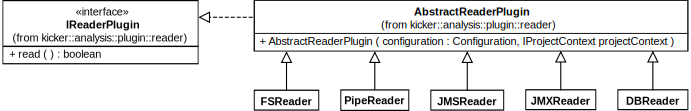
\includegraphics[scale=0.7]{images/kieker_readerimplsuserguide-modified}
\caption{Monitoring reader plugins included with \Kieker{}}
\label{Figure:ReaderHierarchy}
\end{figure}

% \pagebreak

% \
%
% \WARNBOX{This means that whenever a new writer is implemented, a corresponding reader has to be implemented as well. If one want for example to store the recorded informations in a database, one should be capable of reading these saved informations from the database again.}
%
% \

% \enlargethispage{1cm}

\noindent There are already some readers implemented in \Kieker,  as shown in the %
class diagram in Figure \ref{Figure:ReaderHierarchy}. %
The \class{FSReader} has already been used in Section~\ref{sec:example:analysis}. %
The \class{FSReaderRealtime} can be used to simulate continuous monitoring of a %
production system. It adds delays between the delivery of the monitoring records %
to its consumers according to the original delays reconstructed from the logging %
timestamps (Section~\ref{sec:componentsMonitoring:monitoringRecords}).
A brief description of how to use the \class{JMSReader} can be found in Appendix~%
\ref{appendix:usingJMS}. Please note that the database reader (\class{DBReader}) %
is currently in a prototype stage and that it should be used with care. %
Like each plugin, readers are configured via properties, as used in Section~%
\ref{sec:analysis:programmaticCreation} and detailed in Section~%
\ref{sec:analysis:configuration}.

\subsection{Filter Plugins}

Filter plugins receive events (Java objects) via input ports from other %
plugins and implement analyses or visualizations based on these events. %
\Kieker{} already includes some basic filter plugins. For example, the %
\class{CountingFilter} and  \class{TeeFilter} forward incoming events %
to their output ports. The \class{CountingFilter} additionally provides the %
current number of received records via a second output port. The \class{TeeFilter} %
additionally prints incoming events to an output stream, which may be %
the standard output, standard error, a logger, or a file. %
A \class{TimestampFilter} and a \class{TypeFilter} filter incoming records by %
timestamp and by type, respectively. A \class{TraceIdFilter} filters incoming %
trace events (e.g., \class{OperationExecutionRecord}s, see Section~%
\ref{chap:example}) by trace ID. Additional filters for trace analysis, %
architecture reconstruction and visualization are included as part of %
the \KiekerTraceAnalysis{} tool, presented in Chapter~\ref{chap:aspectJ}. %
Like each plugin, filters are configured %
via properties, as used in Section~\ref{sec:analysis:programmaticCreation} and %
detailed in Section~%
\ref{sec:analysis:configuration}. %

% \pagebreak
% \setJavaCodeListing
%\lstinputlisting[caption=MyReponseTimeConsumer.java,label=lst:MyReponseTimeConsumer,firstline=21,firstnumber=21]{\customComponentsBookstoreApplicationDir/src/kieker/examples/userguide/ch3and4bookstore/MyResponseTimeConsumer.java}

% The following Listing~\ref{listing:AnalysisController} shows how to create and run an analysis %
% with these custom components:
%
% \setJavaCodeListing
% \lstinputlisting[caption=Code snippet setting up and running a \KiekerAnalysisPart{} instance (Starter.java),label=listing:AnalysisController,firstline=48, lastline=82, firstnumber=48]%
% {\customComponentsBookstoreApplicationDir/src/kieker/examples/userguide/ch3and4bookstore/Starter.java}

% \enlargethispage{1.2cm}

\subsection{Repositories}

Currently, \Kieker{} includes a single repository, \class{SystemModelRepository}, %
which is used by the \KiekerTraceAnalysis{} filters to update and query %
a component-based system model representing architectural entities %
and structures discovered while processing the incoming monitoring data. %
The development and use of repositories is detailed in Section~%
\ref{sec:analysis:repositories}. %

\section{Developing Analysis Plugins and Repositories}\label{sec:analysis:plugins}

When implementing analysis plugins (i.e., readers or filters) and repositories, %
the classes \class{AbstractReaderPlugin}, \class{AbstractFilterPlugin}, or, %
respectively, \class{AbstractRepository} need to be extended %
(Figure~\ref{fig:analysisController:classdiagram}). %
Section~\ref{sec:analysis:configuration} describes how plugins and repositories %
can be configured via properties. %
Section~\ref{sec:analysis:pluginAnnotation} %
describes how to declare meta-information for plugins using %
dedicated annotations. %
Specific information on the development of custom filters, readers, and repositories %
are given in Sections~\ref{sec:analysis:filters}--\ref{sec:analysis:repositories}. %

% The monitoring record consumer plugins described in the following %
% Section~\ref{sec:analysis:consumer}, are special analysis plugins that receive %
% the monitoring records provided by the monitoring reader. %
% Starting with these monitoring record plugins, analysis plugins can be connected %
% in a pipe-and-filter style to implement more complex analyses. %
% \Kieker{} provides input and output port interfaces and implementing classes %
% to implement such analyses. See the documentation of the classes \class{AbstractInputPort} %
% and \class{OutputPort} for details. \KiekerTraceAnalysis{} is implemented %
% based on this pattern.

\subsection{Configuration}\label{sec:analysis:configuration}

\noindent According to the %
configuration of the \KiekerMonitoringPart{} components (see Section~\ref{sec:monitoring:configuration}),
plugins and repositories are configured via \class{Configuration} objects. Classes must %
provide a public constructor, accepting a \class{Configuration} object as %
its only argument. It is important to invoke the constructor of the super class. %
The configuration properties accepted by a plugin or repository should be provided via \class{public static} %
constants with prefix \method{CONFIG\_PROPERTY\_NAME\_} in order to ease the %
programmatic initialization of plugins (Section~\ref{sec:analysis:programmaticCreation}). %
For the example filter \class{MyResponseTimeFilter},
Listing~\ref{listing:MyResponseTimeFilterConstructor} shows the constructor,
the configuration property, and the corresponding member value obtained from the %
configuration.

\setJavaCodeListing
\lstinputlisting[firstline=43, firstnumber=43, lastline=51, caption={Plugin constructor accepting a \class{Configuration} object}, label=listing:MyResponseTimeFilterConstructor]%
{\customComponentsBookstoreApplicationDir/src/kieker/examples/userguide/ch3and4bookstore/MyResponseTimeFilter.java}

\noindent Additionally, a default configuration and the %
current configuration must be provided via the methods \method{getDefaultConfiguration} and %
\method{getCurrentConfiguration}. Please note that the returned configuration %
must be sufficient to initialize the plugin or repository via the mentioned constructor. %
The \class{AnalysisController} uses the \method{getCurrentConfiguration} to %
save the pipe-and-filter configuration. Listing~\ref{listing:MyResponseTimeFilterEventsToOutput} %
shows how the methods are implemented for the example filter \class{MyResponseTimeFilter}. %

\setJavaCodeListing
\lstinputlisting[firstline=67, firstnumber=67, lastline=72, caption={Plugin returning its default and current configurations}, label=listing:MyResponseTimeFilterEventsToOutput]%
{\customComponentsBookstoreApplicationDir/src/kieker/examples/userguide/ch3and4bookstore/MyResponseTimeFilter.java}


\subsection{@Plugin Annotation and Output Ports}\label{sec:analysis:pluginAnnotation}

\noindent The \class{@Plugin} class annotation is used to define a %
plugin name, a description, and the list of output ports. %
Listing~\ref{listing:MyResponseTimeFilterPluginAnnotationOutputs} shows the %
\class{@Plugin} annotation for the example filter.

If the \class{@Plugin} annotation is not present for a plugin, the \method{name} %
defaults to the plugin's (simple) classname, the \method{description} defaults %
to the empty string, and the list of output ports is empty. These default values %
are also used in case a respective attribute is omitted. %
Note that the name is not required to be a unique among filters; it is simply %
used for descriptive purposes, such as in Figure~\ref{fig:example:pipe-and-filter}. %

Output ports are specified using the nested \class{@OutputPort} annotation. %
In addition to a name and a description for the output port, a list of event %
types can be specified. Note that in this case, the name is mandatory and must %
be unique for a plugin, as it is used for connecting input and output ports. %
The list of event types defaults to a list including only \class{Object.class}. %
The output port names should be provided as a \class{public static} constant %
with prefix \method{OUTPUT\_PORT\_NAME\_}, in order to ease the programmatic %
connection of readers and filters, as described in %
Section~\ref{sec:analysis:programmaticCreation}. Repositories required by %
filters are also specified as part of the \class{@Plugin} annotation. %
This is detailed in Section~\ref{sec:analysis:repositories}. %

\setJavaCodeListing
\lstinputlisting[firstline=26, firstnumber=26, lastline=38, caption={@Plugin annotation for the example plugin \class{MyResponseTimeFilter}}, label=listing:MyResponseTimeFilterPluginAnnotationOutputs]%
{\customComponentsBookstoreApplicationDir/src/kieker/examples/userguide/ch3and4bookstore/MyResponseTimeFilter.java}

\noindent Plugins can send events to their output ports by calling the %
\method{deliver} method provided by the super class. The method expects the %
output port name and the event to be sent as arguments. Listing~%
\ref{listing:MyResponseTimeFilterDelivers} %
shows how the example filter plugin \class{MyResponseTimeFilter} delivers records %
to its two output ports declared in the \class{@Plugin} annotation.

\setJavaCodeListing
\lstinputlisting[firstline=60, firstnumber=60, lastline=64, caption={Plugin sending events to output ports}, label=listing:MyResponseTimeFilterDelivers]%
{\customComponentsBookstoreApplicationDir/src/kieker/examples/userguide/ch3and4bookstore/MyResponseTimeFilter.java}


\subsection{Developing Monitoring Reader Plugins}\label{sec:analysis:reader}

\noindent Custom readers must extend the class %
\class{AbstractReaderPlugin} (see Figure~\ref{fig:analysisController:classdiagram}), %
and implement the methods \method{init}, \method{read}, and \method{terminate}, %
which are called by the \class{AnalysisController} to trigger the reader's initialization, %
reading, and termination. Like each plugin (Section~\ref{sec:analysis:configuration}), %
readers are configured via a constructor accepting a \class{Configuration} object %
as its only argument; they must provide the default and current configurations %
via the implemented \method{getDefaultConfiguration} and \method{getCurrentConfiguration} %
methods. Readers start reading on invocation of the \method{read} method, %
providing the obtained records to connected filters via the output port(s) %
declared in the \class{@Plugin} annotation (Section~\ref{sec:analysis:pluginAnnotation}). %
The \method{read} method should be implemented synchronously, i.e., it should %
return after reading is finished or has been aborted via an invocation of the %
\method{terminate} method.

Listing~\ref{listing:MyPipeReaderPluginAnnotation} shows the \class{@Plugin} %
annotation  of the example reader \class{MyPipeReader}. Reading monitoring %
records from the monitoring pipe introduced in the previous Chapter~%
\ref{sec:monitoring-log-writers}, the reader provides received monitoring %
records via its output port.

% If there is nothing on the pipe to be read, the reader waits 4 seconds at maximum before it terminates.
% \setJavaCodeListing
% \lstinputlisting[firstline=29, firstnumber=29, caption=MyPipeReader.java (excerpt), label=listing:MyReader,float]{\customComponentsBookstoreApplicationDir/src/kieker/examples/userguide/ch3and4bookstore/MyPipeReader.java}

\setJavaCodeListing
\lstinputlisting[firstline=29, firstnumber=29, lastline=40, caption={@Plugin annotation for the example reader}, label=listing:MyPipeReaderPluginAnnotation]%
{\customComponentsBookstoreApplicationDir/src/kieker/examples/userguide/ch3and4bookstore/MyPipeReader.java}

\noindent Listing~\ref{listing:MyPipeReaderInit} shows an excerpt of the \class{MyPipeReader}'s %
constructor. In this case, the reader reads the pipe name from the %
configuration and connects to the named pipe. Optionally, the reader can override the 
\method{init} method.

\setJavaCodeListing
\lstinputlisting[firstline=54, firstnumber=54, lastline=60, caption={Example reader's initialization in the constructor (excerpt)}, label=listing:MyPipeReaderInit]%
{\customComponentsBookstoreApplicationDir/src/kieker/examples/userguide/ch3and4bookstore/MyPipeReader.java}

\pagebreak

\noindent Listing~\ref{listing:MyPipeReaderRead} shows the \class{MyPipeReader}'s %
\method{read} method. In this case, the reader polls the pipe for new records %
and forwards these to its output port.

\setJavaCodeListing
\lstinputlisting[firstline=63, firstnumber=63, lastline=82, caption={Example reader's \method{read} method}, label=listing:MyPipeReaderRead]%
{\customComponentsBookstoreApplicationDir/src/kieker/examples/userguide/ch3and4bookstore/MyPipeReader.java}

\subsection{Developing Filter Plugins}\label{sec:analysis:filters}

Custom filters must extend the class \class{AbstractFilterPlugin}. %
In addition to providing meta information, including output ports, via the %
\class{@Plugin} annotation %
(Section~\ref{sec:analysis:pluginAnnotation}), as well as implementing a constructor %
and getters for handling \class{Configuration}s (Section~\ref{sec:analysis:configuration}), %
filters may override the methods \method{init} and %
\method{terminate} methods, implementing initialization and cleanup tasks. %
The \class{@Plugin} annotation of the example filter \class{MyResponseTimeFilter} %
was shown in Listing~\ref{listing:MyResponseTimeFilterPluginAnnotationOutputs} already.

Filters receive events via methods marked with the \class{@InputPort} %
annotation. These methods must accept a single argument, which has to be %
a super type of the set of accepted event types declared in the respective %
\class{@InputPort} annotation's \method{eventTypes}. %
In addition to an optional \method{description}, each \class{@InputPort} %
must have a \method{name}, which is unique for this filter. The input port names %
should be provided as a \class{public static} constants %
with prefix \method{INPUT\_PORT\_NAME\_}, in order to ease the programmatic %
connection of readers and filters, as described in %
Section~\ref{sec:analysis:programmaticCreation}. %
Listing~\ref{listing:MyResponseTimeFilterInputPort} shows the declaration %
of the input port provided by the example plugin \class{MyResponseTimeFilter}. %
The body of this method was shown in Listing~%
\ref{listing:MyResponseTimeFilterPluginAnnotationOutputs} already.

\pagebreak

\setJavaCodeListing
\lstinputlisting[firstline=55, firstnumber=55, lastline=59, caption={@InputPort annotation for the example plugin's input method}, label=listing:MyResponseTimeFilterInputPort]%
{\customComponentsBookstoreApplicationDir/src/kieker/examples/userguide/ch3and4bookstore/MyResponseTimeFilter.java}

\subsection{Developing and Accessing Required Repositories}\label{sec:analysis:repositories}

Custom repositories must extend the class \class{AbstractRepository}. %
The \class{@Repository} annotation is used to provide a \method{name} %
and a \method{description} for a repository type. %
Listing~\ref{listing:RepositoryAnnotation} shows the \class{@Repository} annotation %
of the \class{SystemModelRepository} which as included in Kieker, as part of the %
\KiekerTraceAnalysis{} tool. %

\setJavaCodeListing
\lstinputlisting[firstline=39, firstnumber=39, lastline=42, caption={\class{@Respository} annotation of Kieker's \class{SystemModelRepository}}, label=listing:RepositoryAnnotation]%
{../../src/tools/kieker/tools/traceAnalysis/systemModel/repository/SystemModelRepository.java}

\noindent Plugins specify the list of required repositories in their %
\class{@Plugin} annotation. Repositories are connected to filter-provided %
repository ports. A plugin's repository ports are specified using the %
nested \class{@RepositoryPort} annotation, as depicted for a %
\KiekerTraceAnalysis{} filter in Listing~\ref{listing:RepositoryRequirementDeclaration}. %
Like for input and output port names, this name must be unique for the plugin %
and should be provided as a \class{public static} constant %
with prefix \method{REPOSITORY\_PORT\_NAME\_}, in order to ease the programmatic %
connection of repositories to readers and filters. %

\setJavaCodeListing
\lstinputlisting[firstline=40, firstnumber=40, lastline=43, caption={Declaration of required repositories in the @Respository annotation}, label=listing:RepositoryRequirementDeclaration]%
{../../src/tools/kieker/tools/traceAnalysis/filter/AbstractTraceAnalysisFilter.java}

\noindent Plugins can access their connected repositories via the \method{getRepository} %
method provided by the super class, as shown in Listing~\ref{listing:RepositoryAccess}. %

\setJavaCodeListing
\lstinputlisting[firstline=147, firstnumber=147, lastline=148, caption={Accessing a repository within in a plugin}, label=listing:RepositoryAccess]%
{../../src/tools/kieker/tools/traceAnalysis/filter/AbstractTraceAnalysisFilter.java}

